\section{Implementation}
\label{sec: implementation}

There are several implementation details that worth mentioning here. 

\subsection{Kinect}
We have purchased two Kinect sensors: one for XBox the other for Windows. Kinect SDK is a Windows-based API allowing us to access the raw depth and RGB images from both versions of Kinect. The Windows version offers a near mode to permit objects to be within 30cm of the Kinect. In the labeling the color gloves to generate training samples, we use the built-in function provided by Kinect SDK to map the color pixel to depth pixel. The color detection turns out not to work very well since there are many noises due to lighting and the camera. However with cropping and depth-thresholding, we managed to labeled hundreds of images. At this time, we did not use the gloves with fingers colored, as we found (1) it is difficult to produce a perfectly built color gloves and (2) the low resolution of the Kinect sensor might not capture the details of figure very well.

\subsection{GPU Implementation}
From a programmer's perspective, GPU is seen as an I/O device: one has to move the data from main memory to the GPU memory and move back the processed data to the main memory. There are several libraries for us to consider to program on GPU: Microsoft DirectX, Microsoft DirectCompute, OpenCL, CUDA. We decided to use OpenCL as it is a standard library for general purpose computing on GPU and can run on almost all GPU (as opposed on CUDA which can only run on NVidia cards). OpenCL is using C as the programming language and has an event-queue framework to process incoming data. 

We have considered the layout of the decision tree in the GPU memory since we found the cache hit is low. Since we store the tree linearly in the memory, we have tested (1) using pre-order traversal (depth first), and (2) breath first traversal for the data structures. It turns out there is no significant difference between the two data structures. So we use the first data structure.  

\subsection{Training Random Forest}

The training samples generated is big, usually more than 10 GB. We customize a random forest library \cite{alglib}, for example via changing the double type to float type to save the memory size by halt. We wish we could have optimize more on the library since we spend some long time on training, e.g., the longest one lasts more than 24 hours. It would be an interesting research topic to parallelize random forest to multi-core and distributed systems.     

We use Amazon Elastic Computing Cloud (EC2) to offload our massive training workloads to cloud servers.  

\subsection{Refinements}
\label{sec:refinement}

Several improvements we found are very important for our systems.

\textbf{Adding a virtual wall.} Our system will be placed in a variety of environments and therefore the background will be drastically variable. We decide to add a virtual wall after 1.5m so every pixel farther than 1.5m is treated as 1.5m. We found this technique can deal with a lot of variability of the backgrounds and make prediction accurate. 

\textbf{Pruning.} To prune a tree we fix a maximum depth to traverse down each tree. Once the node exceeds the maximum depth it becomes a leaf and the label would be the majority labels in the node's sub-tree. Pruning turns out to be crucial for us since it can guarantee the \textit{worst-case} prediction time. Moreover pruning can make the decision tree almost balanced, ensuring the per-pixel prediction is done in almost constant time. Let us denote the maximum depth to be $d_{\text{tree}}$, the run-time complexity can go down to $O(d_{\text{tree}}\times n_{\text{tree}})$.


\subsection{Actual System}

Our main application is written in C\# in Windows, training algorithm is written in C++, and GPU prediction is written in C. The actual system would show three images: color image, depth image with per-pixel classification, pooled image with the largest cluster's position and type. Also the system would report the real-time performance for each stage. An illustrating example is shown in Figure \ref{fig: system}.


\begin{figure}
\centering
	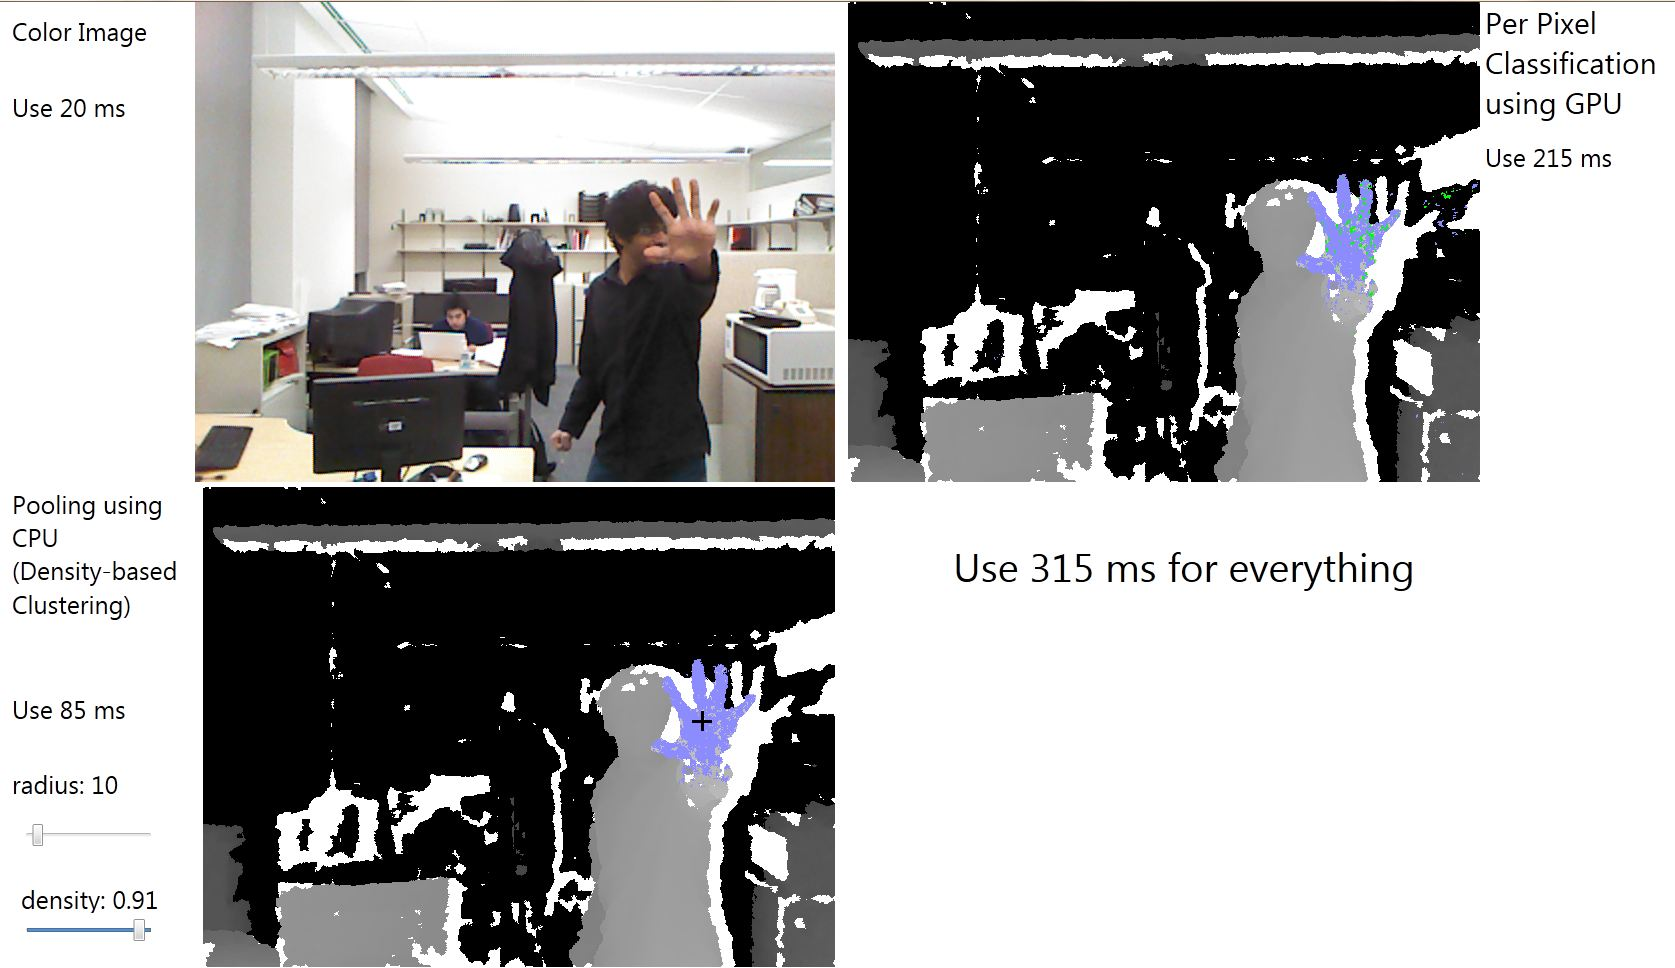
\includegraphics[width=0.5\textwidth]{fig/System.jpg}
	\caption{A snap shot of the actual system. Note the prediction is longer than it is used in a demo machine.}
\label{fig: system}
\end{figure}

We built a demo application that maps two gestures onto mouse state. The location of the hand in the XY plane determined the XY location of the mouse; moving the hand to and from the camera moved the mouse wheel up and down; and closing and opening the hand pressed down and released the left mouse button respectively. This simple mapping enabled us to navigate many applications. We successfully demonstrated this mapping on the Google Earth application \cite{googleearth} by panning and zooming the map.
